\chapter{Oplossingen van de Oefeningen}
\section{Hoofdstuk 1}
\section{Hoofdstuk 2}
\section{Hoofdstuk 3}
\subsection{Karnaugh-kaarten}
\subsubsection{Invullen van Karnaugh-kaarten}
\begin{figure}[hbt]
\centering
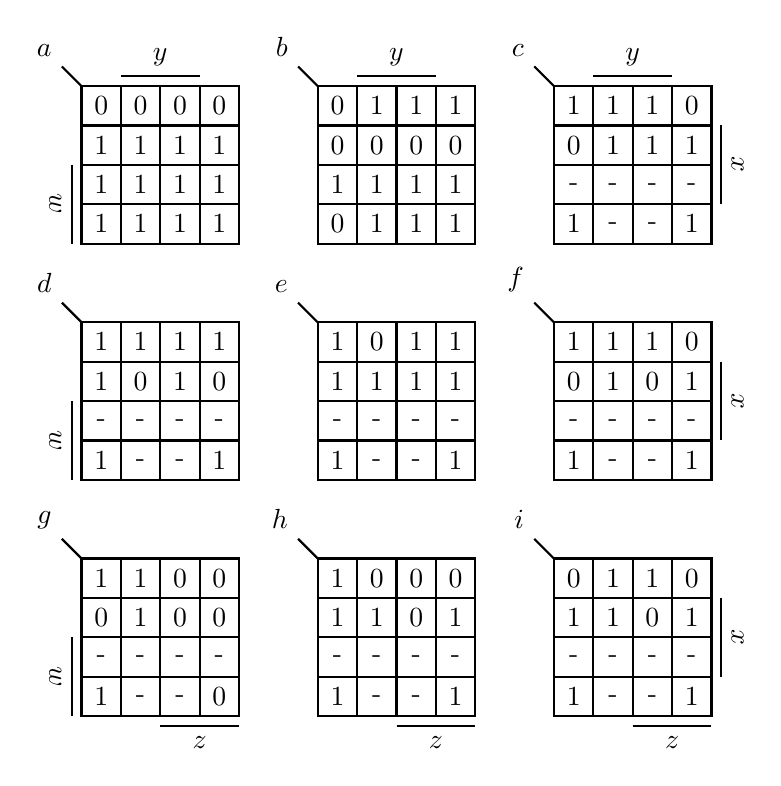
\begin{tikzpicture}
\foreach \x in {-1,0,1} {
  \foreach \y in {-1,0,1} {
    \draw[thick] (-1+3*\x,-1+3*\y) rectangle ++(2,2);
    \draw[thick] (3*\x-0.5,3*\y-1) -- ++(0,2);
    \draw[thick] (3*\x,3*\y-1) -- ++(0,2);
    \draw[thick] (3*\x+0.5,3*\y-1) -- ++(0,2);
    \draw[thick] (3*\x-1,3*\y-0.5) -- ++(2,0);
    \draw[thick] (3*\x-1,3*\y) -- ++(2,0);
    \draw[thick] (3*\x-1,3*\y+0.5) -- ++(2,0);
  }
  \draw[thick] (-4.125,3*\x) to node[midway,below,sloped]{$w$} (-4.125,3*\x-1);
  \draw[thick] (4.125,3*\x+0.5) to node[midway,above,sloped]{$x$} (4.125,3*\x-0.5);
  \draw[thick] (3*\x-0.5,4.125) to node[midway,above,sloped]{$y$} (3*\x+0.5,4.125);
  \draw[thick] (3*\x,-4.125) to node[midway,below,sloped]{$z$} (3*\x+1,-4.125);
}
\foreach \t/\x/\y/\va/\vb/\vc/\vd/\ve/\vf/\vg/\vh/\vi/\vj/\vk/\vl/\vm/\vn/\vo/\vp in {a/-1/-1/0/0/0/0/1/1/1/1/1/1/1/1/1/1/1/1, b/0/-1/0/1/1/1/0/0/0/0/1/1/1/1/0/1/1/1, c/1/-1/1/1/1/0/0/1/1/1/-/-/-/-/1/-/-/1, d/-1/0/1/1/1/1/1/0/1/0/-/-/-/-/1/-/-/1, e/0/0/1/0/1/1/1/1/1/1/-/-/-/-/1/-/-/1, f/1/0/1/1/1/0/0/1/0/1/-/-/-/-/1/-/-/1, g/-1/1/1/1/0/0/0/1/0/0/-/-/-/-/1/-/-/0, h/0/1/1/0/0/0/1/1/0/1/-/-/-/-/1/-/-/1, i/1/1/0/1/1/0/1/1/0/1/-/-/-/-/1/-/-/1} {
  \draw[thick] (3*\x-1,-3*\y+1) -- ++(-0.25,0.25) node[anchor=south east]{$\t$};
  \draw (3*\x-0.75,-3*\y+0.75) node{\va};
  \draw (3*\x-0.25,-3*\y+0.75) node{\vb};
  \draw (3*\x+0.25,-3*\y+0.75) node{\vc};
  \draw (3*\x+0.75,-3*\y+0.75) node{\vd};
  \draw (3*\x-0.75,-3*\y+0.25) node{\ve};
  \draw (3*\x-0.25,-3*\y+0.25) node{\vf};
  \draw (3*\x+0.25,-3*\y+0.25) node{\vg};
  \draw (3*\x+0.75,-3*\y+0.25) node{\vh};
  \draw (3*\x-0.75,-3*\y-0.25) node{\vi};
  \draw (3*\x-0.25,-3*\y-0.25) node{\vj};
  \draw (3*\x+0.25,-3*\y-0.25) node{\vk};
  \draw (3*\x+0.75,-3*\y-0.25) node{\vl};
  \draw (3*\x-0.75,-3*\y-0.75) node{\vm};
  \draw (3*\x-0.25,-3*\y-0.75) node{\vn};
  \draw (3*\x+0.25,-3*\y-0.75) node{\vo};
  \draw (3*\x+0.75,-3*\y-0.75) node{\vp};
}
\end{tikzpicture}
\caption{Oplossingen van het invullen van de Karnaugh-kaarten.}
\label{fig:apxKKaartenFill}
\end{figure}
